\chapter{Vorgehen}


\section{Inbetriebnahme des Vorzeige-Exemplars}
Mit der in der Projektarbeit entwickelten Harvesterschaltung kann per Bluetooth Smart auf dem Android-Endgerät die Geschwindigkeit ausgegeben werden. 


\subsubsection{Reduktion Kapazität Harvesting-Schaltung}
In der Machbarkeitsstudie ist nach dem Gleichrichter ein Kondensator von 470 uF nachgeschaltet. Dieser glätten den Rippel. Ives von EMMicroelectronics rät den Kondensator um den Faktor 10 zu verkleineren, da die nachfolgende Energiemanagementschaltung sonst nicht mit Sicherheit ordnungsgemäss funktioniert. 

Aus diesem Grund wird die Rippelspannung am Ausgangs der Harvesterschaltung mit kleineren Kondensatoren gemessen. Das Messprotokoll befindet sich im Anhang.

Messaufbau




\pagebreak 
\subsubsection{Messungen Energy Management Board}

 
Es zeigt sich, dass der LTS nicht geladen wird . Und es zeigt sich, dass das EM-Board nicht zu regulieren beginnt.

\\

Lastverhalten wie Sensortag

\begin{figure}[h]
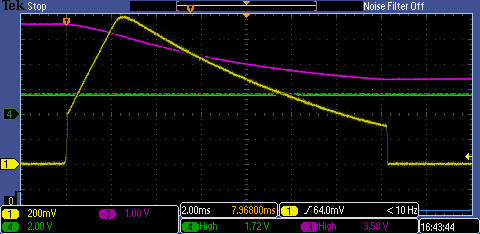
\includegraphics[bb=0 100 50 50]{EMBoardAusgang10Ohm.PNG}
\caption{Ausgangsspannung 10 Ohm}
\end{figure}

\begin{figure}[h]
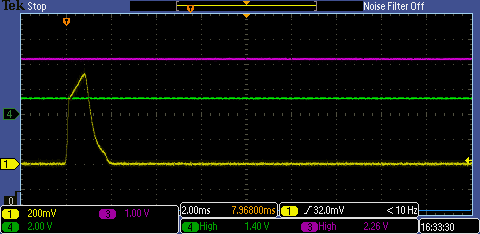
\includegraphics[bb=0 150 50 50]{EMBoardAusgang100Ohm.PNG}
\caption{Energiegewinnung Unbekannte Spule}
\end{figure}



\pagebreak
\subsubsection{Messungen Sensortag}
Ziel: Energieverbrauch kennen.

Unterschied zwischen dem Programmierten Sensortag des Prototypen und dem neuen Sensortag.

\begin{figure}[h]
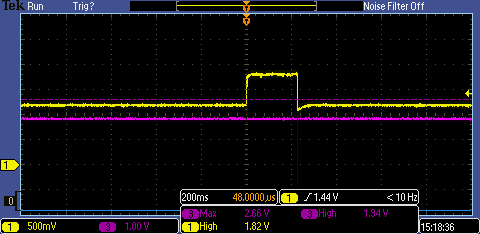
\includegraphics[bb=0 300 50 50]{SensortagRuhestrom.PNG}
\caption{Energieverbrauch (strom) neues Sensortag}
\end{figure}

\begin{figure}[h]
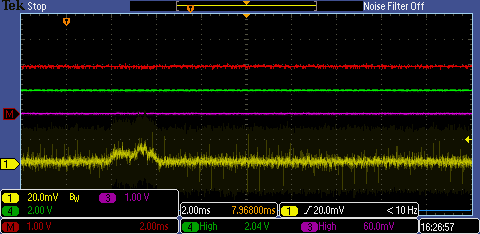
\includegraphics[bb=0 550 50 50]{NeuesSensortagSTromverbrauch.PNG}
\caption{Energieverbrauch Protoyp}
\end{figure}

\textbf{Sensortag Prototyp: defekt ? Auf neues Sensortag Konfiguration neu laden.
}


\section{Layout Print}

\section{Kommunikation Bluetooth Low Energy}

\section{Energieoptimierung}



\section{Applikationsentwicklung}

\section{Option 1}






